\chapter{Conclusion}
brief of conclusion

\section{Conclusion of Problems}
Tell about solving the problem

\section{Conclusion of Method}
Tell about solving using method

\section{Conclusion of Experiment}
Tell about solving in the experiment

\section{Conclusion of Result}
tell about result for purpose of this research.

\section{Andi Muh Aslam/1164064}
\subsection{Teori}
\begin{enumerate}
\item Jelaskan Kenapa Kata-Kata harus dilakukan vektorisasi lengkapi dengan ilustrasi gambar.
\subitem Kata-kata harus dilakukan vektorisasi untuk mengukur nilai kemunculan suatu kata agar dapat di prediksi atau untuk menentukan bobot suatu kata.
\par Untuk ilustrasinya dapat dilihat pada gambar
\begin{figure}[ht]
	\centerline{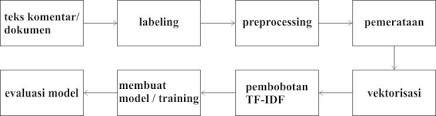
\includegraphics[width=1\textwidth]{figures/andi/L1.PNG}}
	\caption{Ilustrasi Soal No.1}
\end{figure}

\item Jelaskan Mengapa dimensi dari vektor dataset google bisa mencapai 300 lengkapi dengan ilustrasi gambar.
\subitem Dimensi dari vektor dataset google dapat mencapai 300 karena dimensi pada vektor agar dapat membandingkan bobot dari kata tersebut, misalkan terdapat kata Jaket dan Tas pada data set google setiap kata tersebut di buat dimensi vektor senilai 300 kata Jaket dan 300 kata Tas, agar dapat membandingkan bobot dari kesamaan kata Jaket dan Tas. 
\par Untuk ilustrasinya dapat dilihat pada gambar 
\begin{figure}[ht]
	\centerline{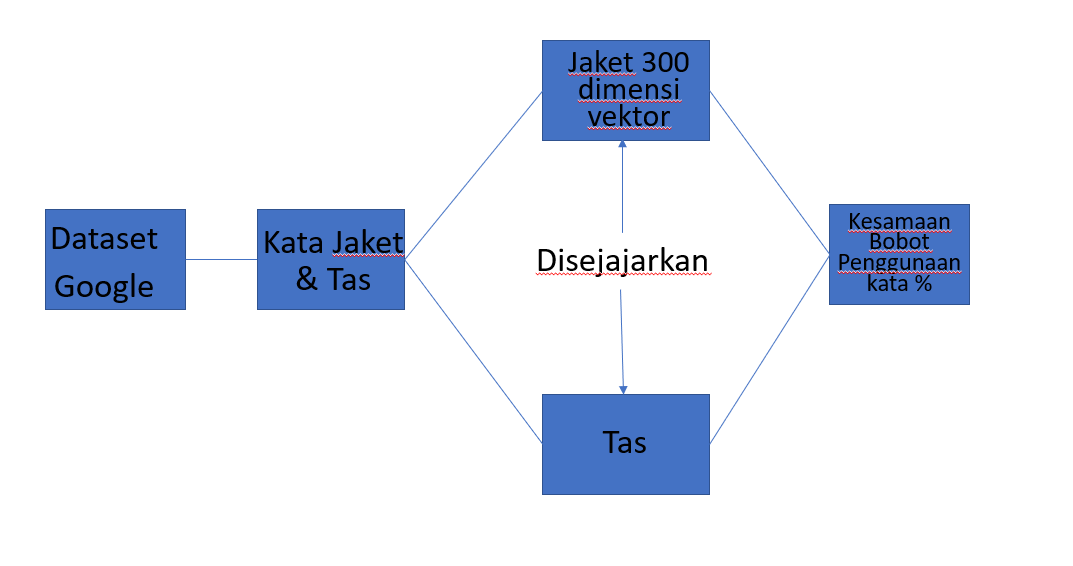
\includegraphics[width=1\textwidth]{figures/andi/L2.PNG}}
	\caption{Ilustrasi Soal No. 2}
	
\end{figure}

\item Jelaskan Konsep vektorisasi untuk kata . dilengkapi dengan ilustrasi atau gambar.
\subitem Konsep dari vektorisasi kata yaitu agar dapat mengetahui kata tengah pada kalimat utama, Contoh ( Subscribe channel ini dan Like yah Guys ). Kata tengah dari contoh tersebut merupakan (dan) yang memiliki bobot sebagai kata tengah dari kalimat. Hal ini sangat berkaitan dengan dimensi vektor pada dataset google karena memiliki nilai atau bobot kata tengah.
\par Untuk ilustrasinya dapat dilihat pada gambar \begin{figure}[ht]
	\centerline{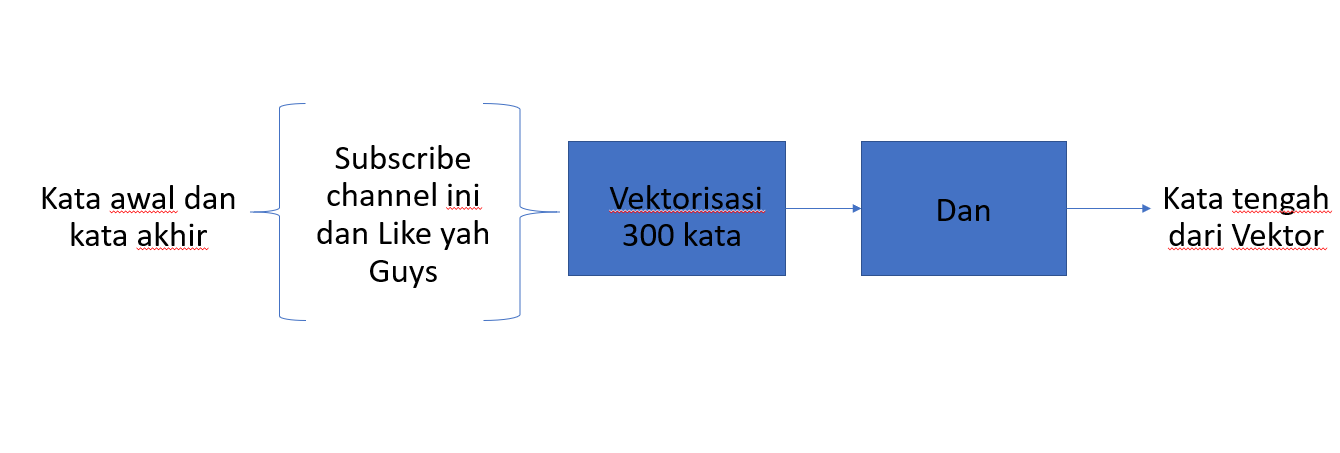
\includegraphics[width=1\textwidth]{figures/andi/L3.PNG}}
	\caption{Ilustrasi Soal No. 3}
	
\end{figure}
\item Jelaskan Konsep vektorisasi untuk dokumen. dilengkapi dengan ilustrasi atau gambar.
\subitem Konsep vektorisasi pada dokumen mesin akan membaca kata-kata terlebih dahulu pada semua kalimat yang ada di dalam dokumen dan nanti kalimat yg ada di dalam dokumen akan dipecah menjadi kata-kata.
\par Untuk ilustrasinya dapat dilihat pada gambar 
\begin{figure}[ht]
	\centerline{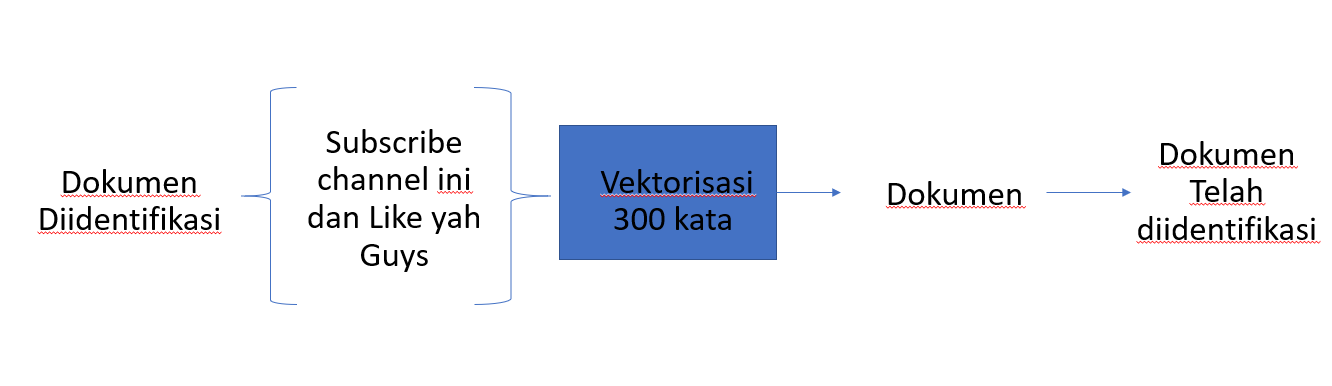
\includegraphics[width=1\textwidth]{figures/andi/L4.PNG}}
	\caption{Ilustrasi Soal No. 4}
	
\end{figure}

\item Jelaskan apa mean dan standar deviasi, lengkapi dengan iludtrasi atau gambar.
\subitem Mean merupakan nilai rata-rata yang tingkat akurasinya tinggi atau nilai tersebut sering munucul. Standar deviasi mengukur bagaimana nilai-nilai data tersebar. Bisa juga didefinisikan sebagai, rata-rata jarak penyimpangan titik-titik data diukur dari nilai rata-rata data tersebut.
\par Untuk ilustrasinya dapat dilihat pada gambar 
\begin{figure}[ht]
	\centerline{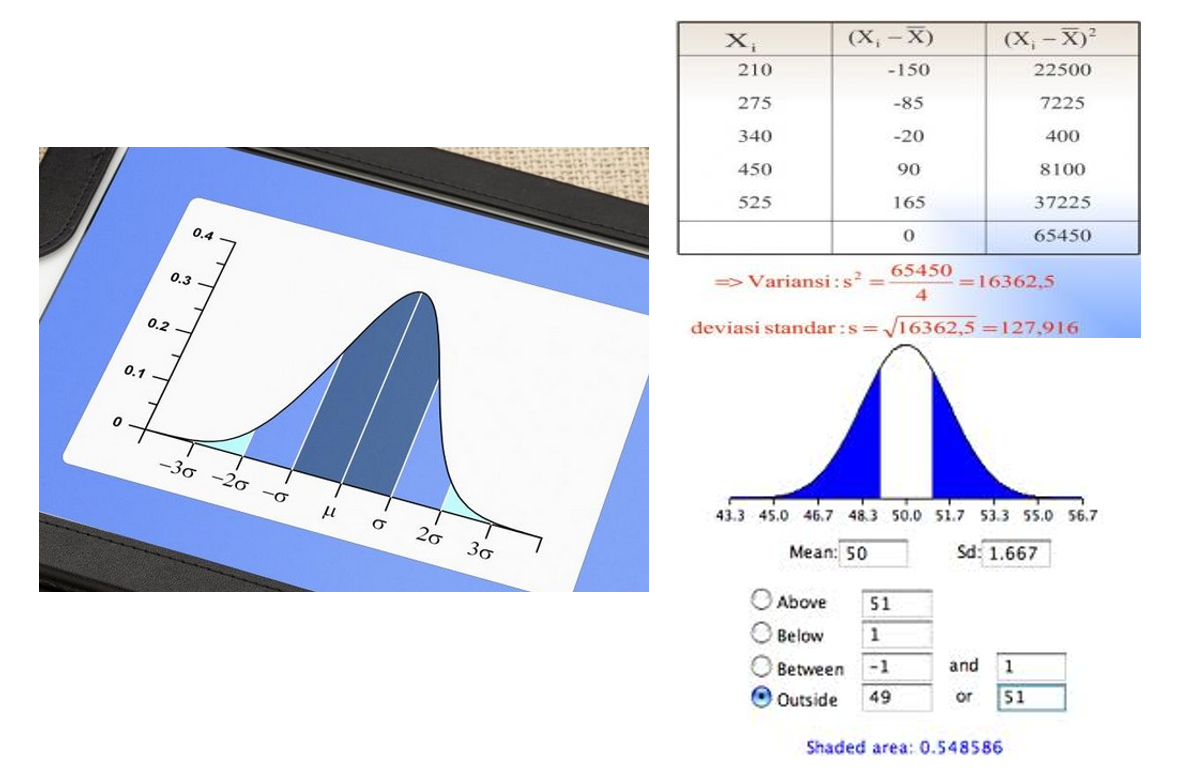
\includegraphics[width=1\textwidth]{figures/andi/L5.PNG}}
	\caption{Ilustrasi Soal No. 5}
	
\end{figure}

\item Jelaskan Apa itu Skip-Gram sertakan contoh ilustrasi.
\subitem Skip-Gram yaitu dimana kata tengah menjadi acuan terhadap kata kata pelengkap dalam suatu kalimat.
\par Untuk ilustrasinya dapat dilihat pada gambar 
\begin{figure}[ht]
	\centerline{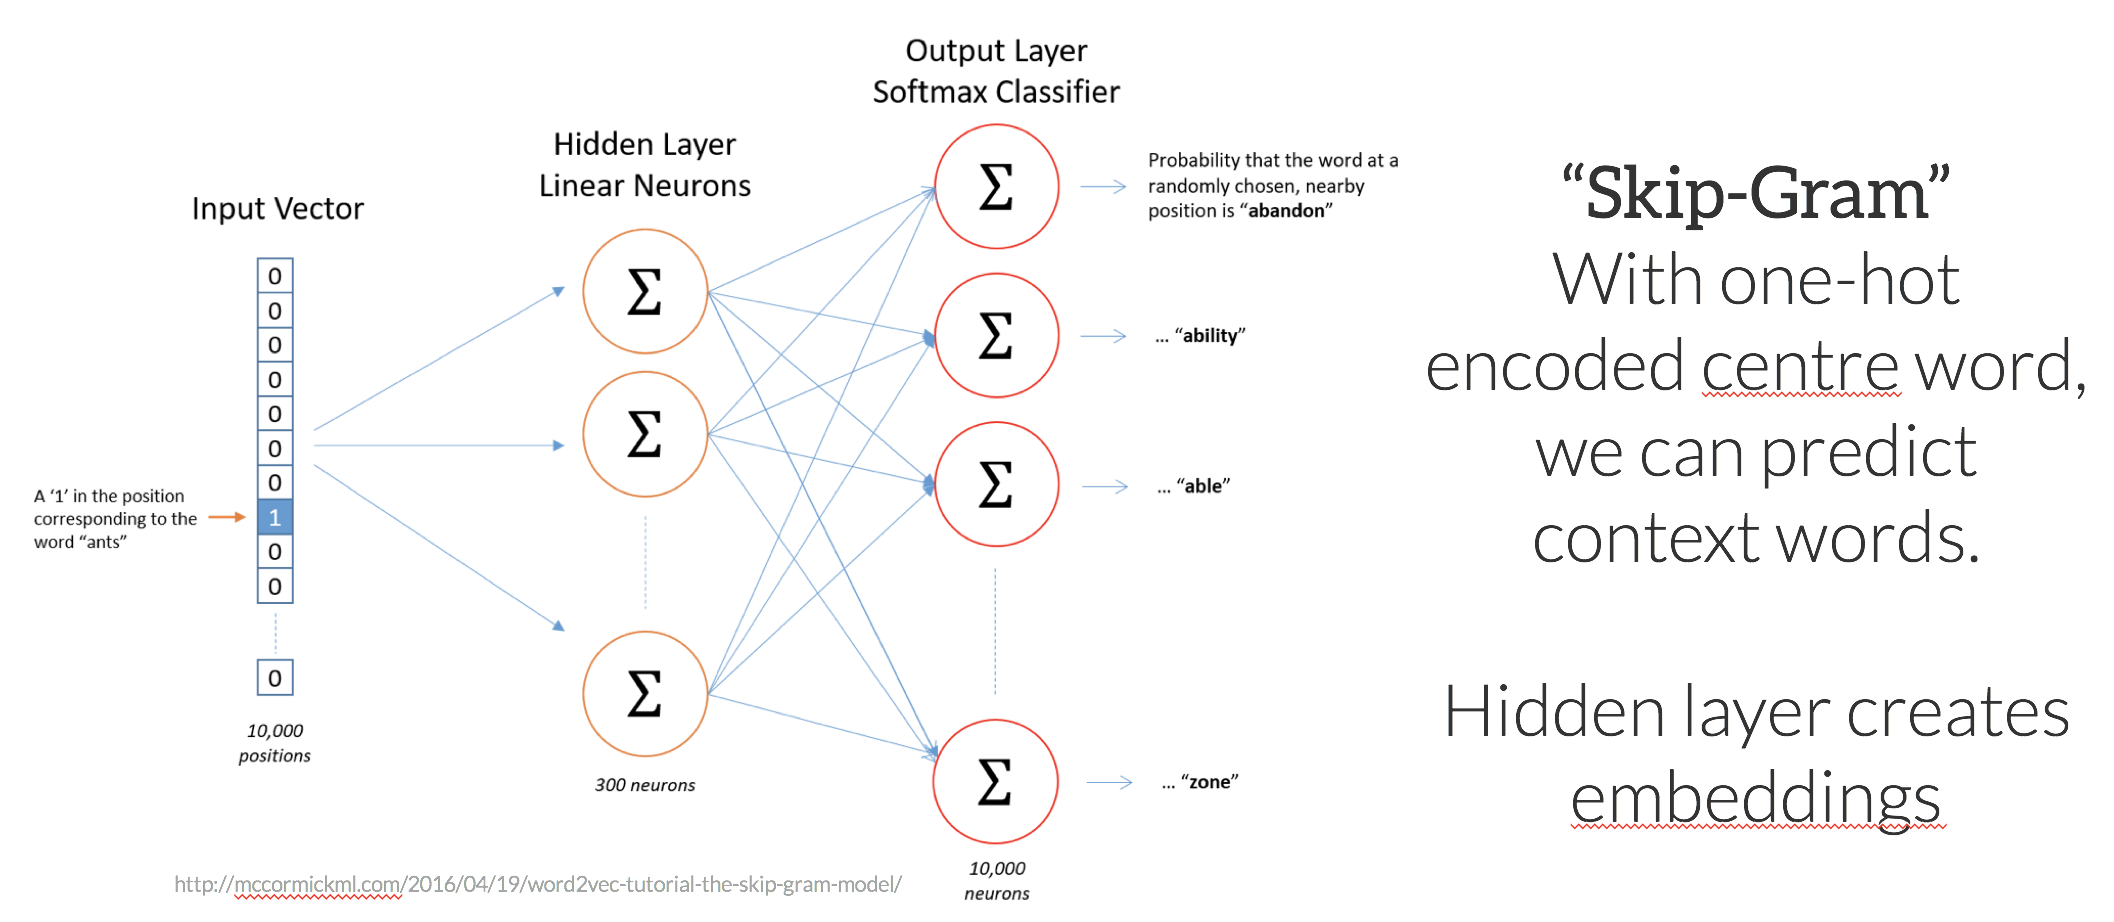
\includegraphics[width=1\textwidth]{figures/andi/L6.PNG}}
	\caption{Ilustrasi Soal No. 6}
	
\end{figure}
\end{enumerate}


\section{Aip Suprapto Munari/1164063}
\subsection{Teori}
\begin{enumerate}

\item Mengapa Kata-Kata Harus di Vektorisasi
\par Kata harus divektorisasi karena mesin hanya mampu membaca data dalam tipe/bentuk angka. Oleh sebab itu, diperlukannya vektorisasi kata untuk mampu mebaca data tersebut. 
\par
\begin{itemize}
\item Gambar :
\par Penjelasan : Berdasarkan pengertian diatas, ada beberapa contoh yang bisa diterapkan. Untuk salah satu contoh dari klasifikasi data sendiri dapat diliat pada gambar berikut \ref{vektorisasikata}.
\begin{figure}[ht]
\centering
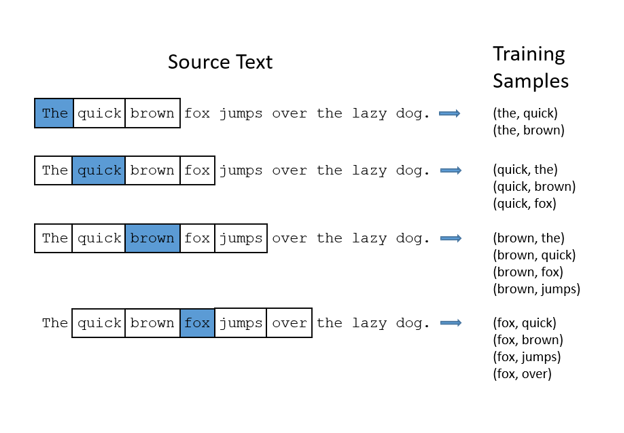
\includegraphics[scale=0.6]{figures/AIP/d1.PNG}
\caption{Vektorisasi Kata Aip}
\label{text-Aip}
\end{figure}
\end{itemize}

\item Mengapa Dimensi Dari Vektor Dataset Google Bisa Sampai 300
\par Setiap nilai dalam vektor 300 dimensi yang terkait dalam sebuah kata "dioptimalkan" dalam  beberapa hal untuk menangkap aspek yang  berbeda. Dengan kata lain masing-masing dari 300 nilai sesuai dengan beberapa fitur abstrak kata. Menghapus kombinasi nilai-nilai ini secara acak akan menghasilkan vektor yang mungkin kurang informasi penting tentang kata tersebut dan mungkin tidak lagi berfungsi sebagai representasi yang baik dari kata itu. Atau singkat cerita mungkin ada lebih dari 3 miliar kata-kata dan kalimat atau data yang tidak mungkin disimpan dalam 1 dimensi vektor maka disimpan menjadi 300 dimensi vektor untuk mengurangi kegagalan memori.
\par
\begin{itemize}
\item Gambar :
\par Penjelasan : Berdasarkan pengertian diatas, ada beberapa contoh yang bisa diterapkan. Untuk salah satu contoh dari klasifikasi data sendiri dapat diliat pada gambar berikut \ref{googleDataset}.
\begin{figure}[ht]
\centering
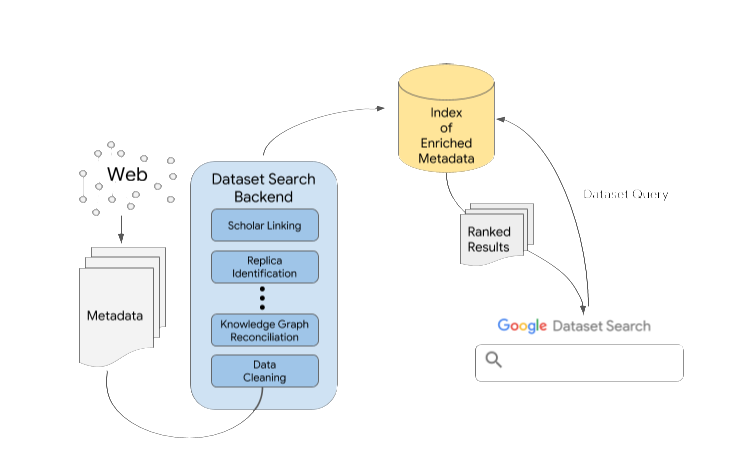
\includegraphics[scale=0.16]{figures/AIP/d2.PNG}
\caption{Google Dataset Aip}
\label{text-Aip}
\end{figure}
\end{itemize}

\item Konsep Vektorisasi Kata 
\par Konsep vektorisasi data merupakan kata-kata yang di inputkan pada mesin learning. Dan outputan nya berupa kara-kata atau keyword dari pencarian yang telah di lakukan sebelumnya. Contoh nya pada saat kita melakukan pencarian di youtube maupun pencarian google. Maka akan muncul hasil dari pencarian dari kata-kata yang telah kita cari atau input.
\par
\begin{itemize}
\item Gambar :
\par Penjelasan : Berdasarkan pengertian diatas, ada beberapa contoh yang bisa diterapkan. Untuk salah satu contoh dari klasifikasi data sendiri dapat diliat pada gambar berikut \ref{vekktorisasikata}.
\begin{figure}[ht]
\centering
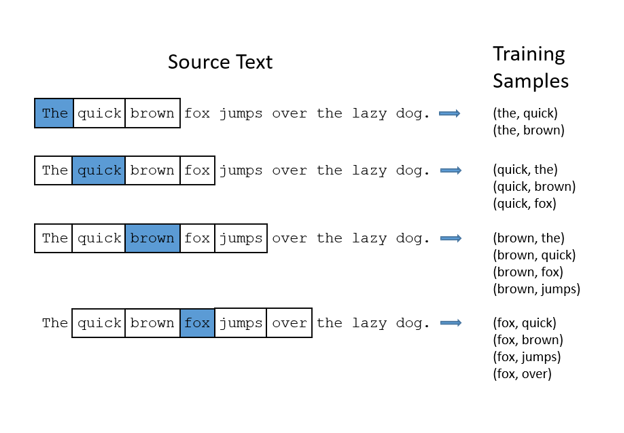
\includegraphics[scale=0.3]{figures/AIP/d1.PNG}
\caption{Vektorisasi Kata Aip}
\label{text-Aip}
\end{figure}
\end{itemize}

\item Konsep Vektorisasi Dokumen 
\par Konsep vektorisasi dokumen yaitu mesin akan membaca terlebih dahulu semua kalimat yang berada pada dalam dokumen dan nanti kalimat tersebut akan di pecah menjadi kata-kata.
\par
\begin{itemize}
\item Gambar :
\par Penjelasan : Berdasarkan pengertian diatas, ada beberapa contoh yang bisa diterapkan. Untuk salah satu contoh dari klasifikasi data sendiri dapat diliat pada gambar berikut \ref{vektorisasidokumen}.
\begin{figure}[ht]
\centering
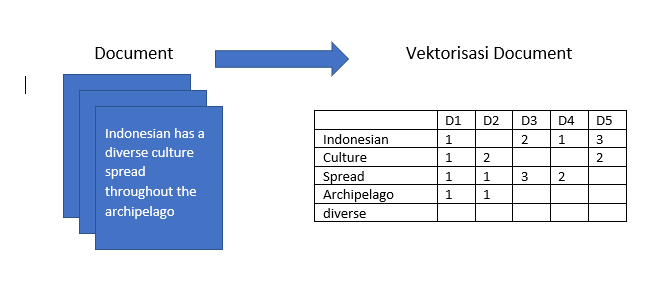
\includegraphics[scale=0.3]{figures/AIP/d3.PNG}
\caption{Vektorisasi Dokumen Aip}
\label{text-Aip}
\end{figure}
\end{itemize}

\item Mean dan Standar Deviasi
\par Mean adalah teknik penjelasan kelompok yang didasarkan atas nilai rata-rata dari kelompok tersebut. Rata-Rata (mean) ini didapat dengan menjumlahkan data seluruh individu dalam kelompok itu, kemudian dibagi dengan jumlah individu yang ada pada kelompok tersebut. Standar deviasi adalah nilai statistik yang digunakan untuk menentukan bagaimana sebaran data dalam sampel, dan seberapa dekat titik data individu ke mean atau rata-rata nilai sampel.Sebuah standar deviasi dari kumpulan data sama dengan nol menunjukkan bahwa semua nilai-nilai dalam himpunan tersebut adalah sama. Sebuah nilai deviasi yang lebih besar akan memberikan makna bahwa titik data individu jauh dari nilai rata-rata.
\par
\begin{itemize}
\item Gambar :
\par Penjelasan : Berdasarkan pengertian diatas, ada beberapa contoh yang bisa diterapkan. Untuk salah satu contoh dari klasifikasi data sendiri dapat diliat pada gambar berikut \ref{mean dan Standar Deviasi}.
\begin{figure}
\centering
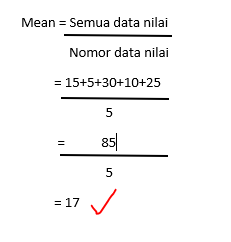
\includegraphics[scale=0.2]{figures/AIP/d4.PNG}
\caption{Mean Aip}
\label{text-Aip}
\end{figure}
\begin{figure}[ht]
\centering
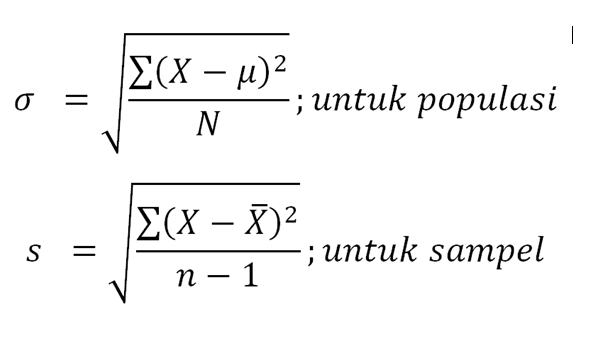
\includegraphics[scale=0.2]{figures/AIP/d5.PNG}
\caption{Standar Deviasi Aip}
\label{text-Aip}
\end{figure}
\par
\end{itemize}

\item Skip Gram
\par Skip-Gram mencoba memprediksi vektor kata-kata yang ada di konteks diberikan vektor kata tertentu. Skip-gram membuat sepasang kata target dan konteks sebagai sebuah instance.
\par
\begin{itemize}
\item Gambar :
\par Penjelasan : Berdasarkan pengertian diatas, ada beberapa contoh yang bisa diterapkan. Untuk salah satu contoh dari klasifikasi data sendiri dapat diliat pada gambar berikut \ref{skipgram}.
\begin{figure}[ht]
\centering
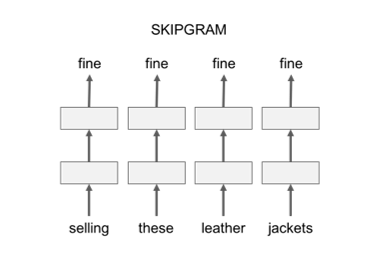
\includegraphics[scale=0.2]{figures/AIP/d6.PNG}
\caption{Skip-Gram Aip}
\label{text-Aip}
\end{figure}
\end{itemize}
\end{enumerate}


\section{PRAKTEK PROGRAM}
\section{Aip Suprapto Munari/1164063}
\subsection{Mencoba Dataset}
\subsubsection{Vektor}
\begin{itemize}
\item Pada gambar diatas dapat dilihat bahwa vektor memiliki array sebanyak 300 dimensi. Untuk identitas sektor satu adalah 0.080
\begin{figure}[ht]
\centering
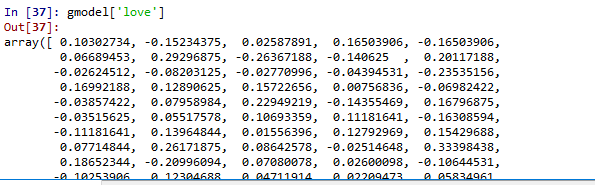
\includegraphics[scale=0.5]{figures/AIP/e4.PNG}
\caption{Vektor Love Aip}
\label{Praktek}
\end{figure}


\item Pada gambar diatas untuk vektor faith dapat dilihat memliki nilai 0.049 , untuk similaritasnya cukup mendekati vektor love dimana faith dapat dikategorikan dalam satu kategori dengan love.
\begin{figure}[ht]
\centering
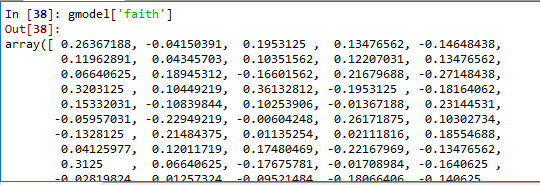
\includegraphics[scale=0.5]{figures/AIP/e5.PNG}
\caption{Vektor Faith Aip}
\label{Praktek}
\end{figure}


\item Vektor fall hanya memiliki nilai yaitu 0.046, dimana mesin memahami bahwa fall terdapat dalam satu kategori yang sama dengan  faith.
\begin{figure}[ht]
\centering
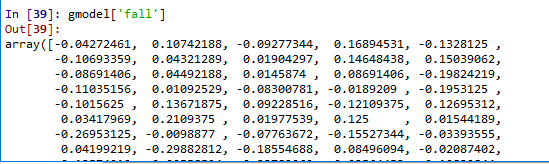
\includegraphics[scale=0.5]{figures/AIP/e6.PNG}
\caption{Vektor Fall Aip}
\label{Praktek}
\end{figure}


\item  Vektor sick memiliki nilai identitas 0.085 dimana mendekati love.
\begin{figure}[ht]
\centering
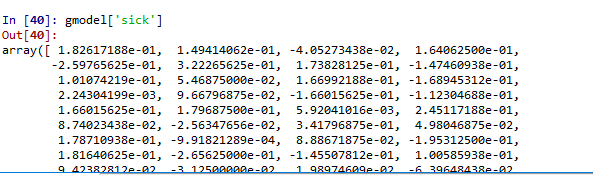
\includegraphics[scale=0.5]{figures/AIP/e7.PNG}
\caption{Vektor Sick Aip}
\label{Praktek}
\end{figure}


\item Vektor clear memiliki nilai identitas -0,025 dan tidak mendekati nilai dari vektor manapun sehingga tidak dapat dijadikan dalam satu kategori.
\begin{figure}[ht]
\centering
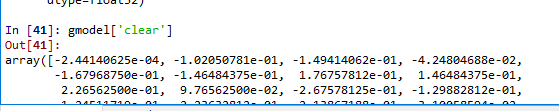
\includegraphics[scale=0.3]{figures/AIP/e8.PNG}
\caption{Vektor Clear Aip}
\label{Praktek}
\end{figure}

\item Untuk vektor shine 0.35 mendekati vektor Faith dan fall.
\begin{figure}[ht]
\centering
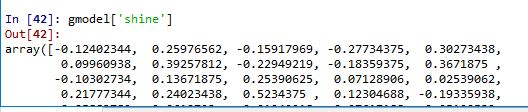
\includegraphics[scale=0.3]{figures/AIP/e9.PNG}
\caption{Vektor Shine Aip}
\label{Praktek}
\end{figure}


\item Vektor bag memiliki i=nilai identitas 0.026 yang mendekati dengan vektor fall dan faith. Sehingga mesin memahami bahwa mungkin saja kedua vektor tersebut berada dalam satu kategori.
\begin{figure}[ht]
\centering
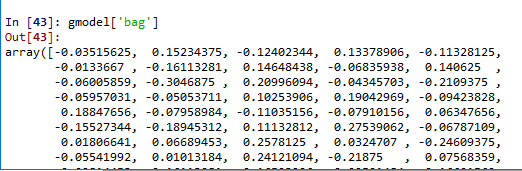
\includegraphics[scale=0.3]{figures/AIP/e10.PNG}
\caption{Vektor Bag Aip}
\label{Praktek}
\end{figure}


\item Vektor car nilainya 0.48 tidak ada yang mendekati vektor manapun sehingga tidak dapat dikategorikan dalam satu kategori.
\begin{figure}[ht]
\centering
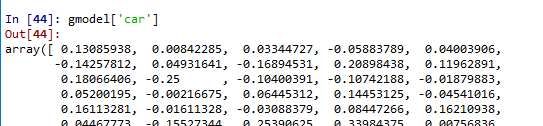
\includegraphics[scale=0.3]{figures/AIP/e11.PNG}
\caption{Vektor Car Aip}
\label{Praktek}
\end{figure}


\item Vektor wash memiliki nilai 0.102 jauh dari vektor vektor lainnya.
\begin{figure}[ht]
\centering
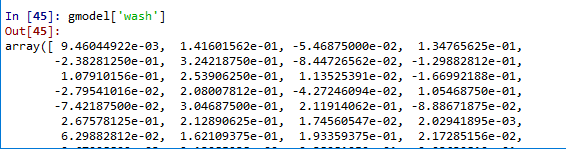
\includegraphics[scale=0.3]{figures/AIP/e12.PNG}
\caption{Vektor Wash Aip}
\label{Praktek}
\end{figure}


\item Vektor cycle memiliki nilai identitas 0.179 yang bisa mendekati vektor wash. Dapat dikatakan bahwa motor dapat dicuci jika diarti dalam satu kategori yang sama.
\begin{figure}[ht]
\centering
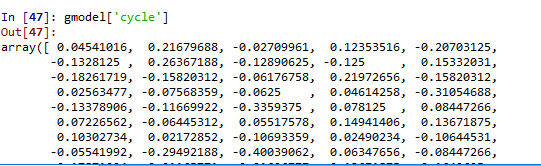
\includegraphics[scale=0.3]{figures/AIP/e14.PNG}
\caption{Vektor cycle Aip}
\label{Praktek}
\end{figure}
\end{itemize}

\subsubsection{Similariti}
\begin{enumerate}
\item Lihat gambar berikut yang merupakan hasil prediksi similariti
\begin{figure}[ht]
\centering
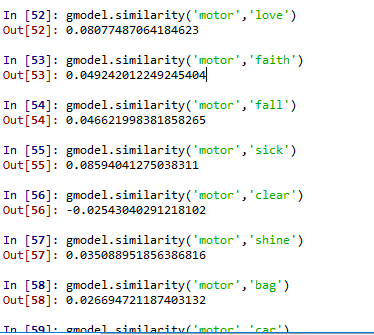
\includegraphics[scale=0.3]{figures/AIP/e17.PNG}
\caption{Similariti Aip}
\label{Praktek}
\end{figure}

Dapat disimpulkan bahwa
\begin{itemize}
\item Untuk Motor dan faith hasilnya adalah 0.049
\item Untuk Motor dan fall hasilnya adalah 0.046
\item Untuk Motor dan clear hasilnya adalah -0.025
\item Untuk Motor dan wash hasilnya adalah 0.102
\item Untuk Motor dan cycle hasilnya adalah 0.179
\item Artinya Motor dan cycle memang dalam kategoriy ang sama misalnya dalam kategori kendaraan. Mesin sudah mengetahui bahwa keduanya dapat dikategorikan sebagai kendaraan.
\end{itemize}
\end{enumerate}

\subsection{Extract Words dan PermuteSentences}
\subsubsection{Extract Words}
ExtractWords merupakan function untuk menambahkan, menghilangkan atau menghapuskan, hal hal yang tidak penting atau tidak perlu di dalam teks. Dalam contoh dibawah ini. menggunakan function extract words untuk menghapus komen dengan python style , mencari data yang diinginkan, dan memberikan spasi pada teks.
\begin{figure}[ht]
\centering
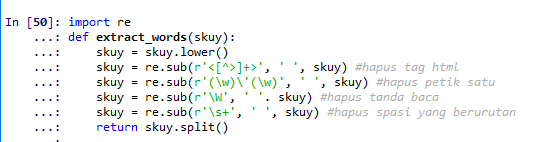
\includegraphics[scale=0.3]{figures/AIP/e15.PNG}
\caption{Extract Words Aip}
\label{Praktek}
\end{figure}

\subsubsection{PermuteSentences}
PermuteSentences merupakan class yang digunakan untuk melakukan pengocokan secara acak pada data yang ada. Digunakan cara ini agar tidak terjadi kelebihan memori pada saat dijalankan. Contoh dibawah yaitu fungsi akan memanggil lenght. Yang kemudian mendefinisikan variabel req untuk lenght dam melakukan random choice yaitu pengocokan acak untuk kata motor.
\begin{figure}[ht]
\centering
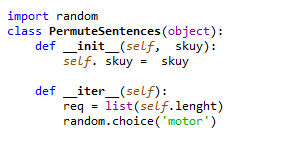
\includegraphics[scale=0.3]{figures/AIP/e16.PNG}
\caption{PermuteSentencesi Aip}
\label{Praktek}
\end{figure}

